\documentclass[12pt,a4paper]{article}

% Paquetes de configuración del documento
\usepackage[utf8]{inputenc}
\usepackage[spanish]{babel}
\usepackage[T1]{fontenc}
\usepackage[margin=2.5cm]{geometry}
\usepackage{fancyhdr}
%Paquetes para simbologia%
\usepackage{amsmath}
\usepackage{amsfonts}
\usepackage{amssymb}
\usepackage{physics}
\usepackage{longtable}
\usepackage{graphicx}
\usepackage{caption}
\usepackage{float}
\usepackage{xurl}
\usepackage[colorlinks=true,
            linkcolor=black,
            urlcolor=myblue,
            citecolor=black,
            filecolor=black]{hyperref}
 % Opción estándar para enlaces
\Urlmuskip=0mu plus 1mu          % Mejora el espaciado para permitir cortes
\usepackage{subcaption}  % en el preámbulo
\usepackage{pgfplots}
\pgfplotsset{compat=1.18}
\usepackage{tikz}
\usepackage{xcolor}
\definecolor{myblue}{RGB}{42, 127, 179}

\pagestyle{fancy}
\chead{\textit{Materiales Metálicos}}
\rhead{\textit{UTN-FRVM}}
\lhead{\textit{Ingeniería Mecánica}}

\begin{document}
\begin{titlepage}
	
	\begin{center}
		{\huge \textit{Universidad Tecnológica Nacional}}\\
        \vspace{0.5cm}
		{\LARGE \textit{Facultad Regional Villa María}}\\
		\vspace{1.5cm}
        {\LARGE{\textit{Ingeniería Mecánica - Materiales Metálicos}}}\\
		\vspace{1.5cm}
        \LARGE{\textit{Trabajo Práctico 3-06}}
	\end{center}
	
	\vfill

    \textit{Grupo DEL RÍO:}
	\begin{itemize}
		\item \textit{Abregú, Iván.}
		\item \textit{Antico, Rodrigo.}
		\item \textit{Brussa,Julián.}
		\item \textit{Cabral, Franco.}
        \item \textit{Cárdenas, Felipe.}
        \item \textit{Cardozo, Martín.}
        \item \textit{Córdoba, Nathan.}
        \item \textit{Cucco, Ramiro.}
        \item \textit{del Río, Juan.}
        \item \textit{Guerini, Nazareno.}
        \item \textit{Medina, Ivo.}
        \item \textit{Ortiz, Gastón.}
        \item \textit{Picos, Elías.}
        \item \textit{Quinteros, Lautaro.}
	\end{itemize}
    
	\textit{Docentes:}
	\begin{itemize}
		\item \textit{Dr. Lucioni, Eldo José.}
		\item \textit{Ing. Victorio Vallaro, Juan Manuel.}
	\end{itemize}
	\centering
	\today
	
\end{titlepage}

\newpage
\tableofcontents

\begin{abstract}
    Analice, investigue e interprete el contenido relacionado con los Casos de Estudio de la bibliografía que se indica a continuación a fin de adquirir efectuar una explicación detallada de los mismos. Adicionalmente, debe emplear Matlab y Python para estar en capacidad de determinar los efectos de la variación de los requerimientos iniciales y de los valores de las propiedades en el modelo de solución adoptado. [NOTA: Anualmente la Cátedra asignará los Casos de Estudio a cada equipo de trabajo].
    \begin{itemize}
        \item Software. \{MM-CAD-TP 3-06\}.
        \item Ashby, M.F. y Jones, D.R.H. Materiales para Ingeniería 2. 1ra Edición. 2009. Cap. 13 Casos prácticos con aceros. \{MM-CAD-0.0.0\}.
        \begin{itemize}
            \item 13.1 Investigación metalúrgica después de la explosión de una caldera (1*) [Caso 2025].
        \end{itemize}
    \end{itemize}
\end{abstract}

\section{Propósito y Fundamento del Caso de Estudio}
Este caso práctico tiene como finalidad comprender cómo los fenómenos metalúrgicos y mecánicos influyen en la falla de componentes de servicio a alta temperatura. 
Se estudiará la rotura de un tubo de caldera de acero al carbono sometido a presión interna y temperaturas elevadas, con el fin de relacionar la microestructura obtenida, las propiedades mecánicas y el mecanismo de fallo observado.

\section{Análisis Metalúrgico del Caso}
La tubería estudiada estaba fabricada en un acero de bajo carbono (Fe-0,18\%C, 0,45\%Mn, 0,20\%Si).
Bajo condiciones normales debería presentar microestructura de ferrita + perlita (dureza $\approx 1.5$ GPa).
El análisis del tubo roto evidenció:
\begin{itemize}
    \item En el borde de la rotura: dureza $\approx$ 4 GPa $\rightarrow$ martensita (producto de enfriamiento muy rápido).
    \item En el interior: dureza $\approx$ 2.2 GPa $\rightarrow$ bainita (enfriamiento intermedio).
\end{itemize}
Esto indica que la tubería se sobrecalentó por encima de la temperatura crítica $A_3 \approx 870^{\circ}$C y sufrió un enfriamiento brusco durante la explosión, generando una microestructura templada.

Las posibles causas del sobrecalentamiento local fueron:
\begin{enumerate}
    \item Formación de depósitos de incrustaciones (agua dura) en la pared interna, actuando como aislante térmico.
    \item Alteraciones en la convección natural, generando una película de vapor seco que impidió el enfriamiento.
\end{enumerate}

\section{Modelo Matemático Adoptado}
El modelo de fluencia utilizado se basa en la ecuación simplificada:

\begin{equation}
    t_r = A \, \sigma^{-n} \, e^{\frac{Q}{R T}}
\end{equation}

donde:
\begin{itemize}
    \item $t_r$ = tiempo a rotura (s).
    \item $\sigma$ = tensión circunferencial de la tubería (MPa).
    \item $T$ = temperatura absoluta (K).
    \item $R = 8.314 \, J/mol\cdot K$.
    \item $Q = 240 \, kJ/mol$ (energía de activación).
    \item $n = 4$ (exponente de tensión).
    \item $A$ = constante calibrada para cumplir que a 900 °C y $\sigma=50$ MPa $\rightarrow$ $t_r \approx 15$ min.
\end{itemize}

La tensión circunferencial se estima como:

\begin{equation}
    \sigma = \frac{p \, r}{t}
\end{equation}

donde $p$ es la presión interna, $r$ el radio del tubo y $t$ el espesor de pared.

\section{Resultados de Simulación}
Se realizaron simulaciones en \textbf{Python} y \textbf{MATLAB} utilizando los scripts \texttt{creep\_model\_full.py} y \texttt{creep\_model\_full.m}.
Se generaron las siguientes gráficas:

\begin{figure}[H]
    \centering
    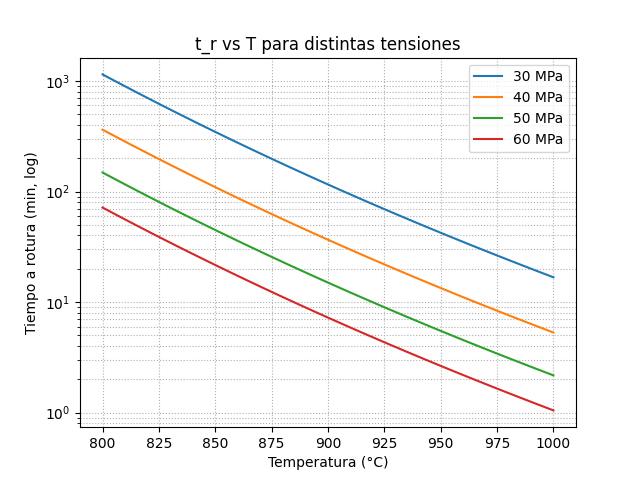
\includegraphics[width=0.7\linewidth]{tr_vs_T.png}
    \caption{Tiempo a rotura en función de la temperatura para distintas tensiones.}
\end{figure}

\begin{figure}[H]
    \centering
    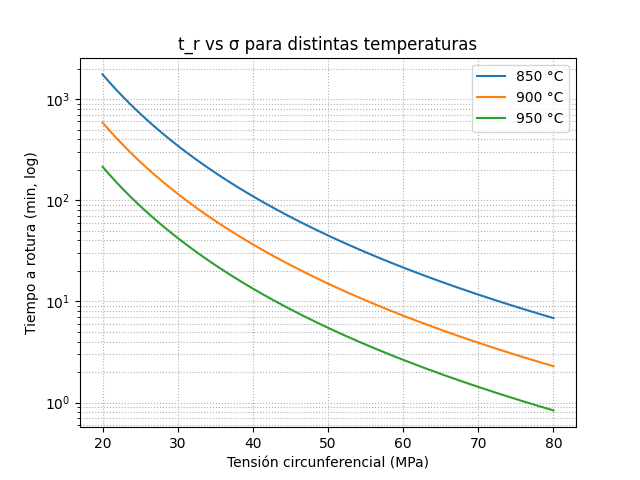
\includegraphics[width=0.7\linewidth]{tr_vs_sigma.png}
    \caption{Tiempo a rotura en función de la tensión circunferencial a distintas temperaturas.}
\end{figure}

\begin{figure}[H]
    \centering
    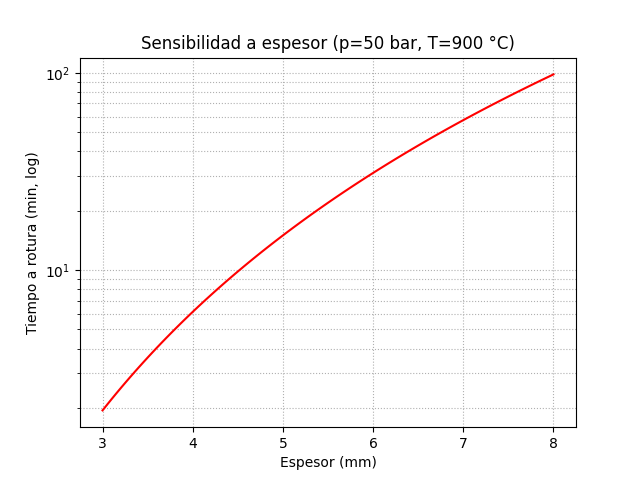
\includegraphics[width=0.7\linewidth]{sens_espesor.png}
    \caption{Sensibilidad del tiempo a rotura con respecto al espesor de pared.}
\end{figure}

\begin{figure}[H]
    \centering
    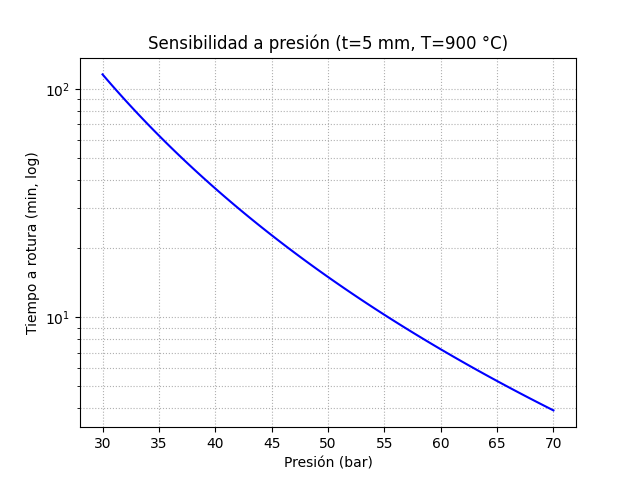
\includegraphics[width=0.7\linewidth]{sens_presion.png}
    \caption{Sensibilidad del tiempo a rotura con respecto a la presión interna.}
\end{figure}

\section{Conclusiones}
\begin{itemize}
    \item La falla del tubo se debió a un episodio de sobrecalentamiento local que llevó al acero a superar los 870 °C, transformándose a austenita.
    \item La brusca liberación de presión provocó un enfriamiento rápido, generando martensita y bainita en la zona afectada.
    \item El modelo de fluencia muestra que a 900 °C y $\sigma \approx 50$ MPa, el tiempo a rotura esperado es de minutos, coherente con el caso real.
    \item Variaciones en espesor y presión modifican fuertemente la vida en servicio, evidenciando la importancia del diseño seguro.
\end{itemize}

\vfill
\textit{\textbf{Este trabajo fue elaborado con la ayuda de la IA y otras páginas de ayuda para facilitar la confección y disposición de los elementos en dicho trabajo.}}

\end{document}